\section{Concepts of Electron Optics}
\label{sec: electron_optics}

Before going into detailed descriptions of different electron microscopes, it is useful to summarize general concepts of electron optics. This involves the definition of properties of an ideal image, principles in imaging with electrons and defects and their corrections of electron lenses.

\subsection{Properties of an Ideal Image}

According to James Clark Maxwell, the quality of an image can be defined by fulfilling three requirements that ensure close resemblance of the image to the corresponding object. These requirements can be taken for characterization of image defects as well for a description for negative examples as follows.\\

The first requirement is that each point in an image, there should be an equivalent point in the object. This requirement is determined by the properties of the optical system. Negative examples would be incorrect focus strength leading to an image formed out of focus. Even at optimal focus strength, aberrations of the lenses could still lead to blurred images with a loss of spatial resolution. Maxwell's second requirement states that the object and the image should exhibit similar geometry meaning that they should show similar patterns of points. Hence, the requirements demands similar geometrical sense, but different orientation or inversion is allowed. Real images can show distortions that correlate to a positional variation of the magnification. Figure \ref{fig: commonDistortions} shows three common distraction types: pincushion distortion (a), barrel distortion (b) and spiral distortion. Pincushion distortion results by an increasing magnification with radial distance from the optic axis, whereas barrel distortion corresponds to a decreasing magnification away from the optic axis. Spiral distortion results, if rotation of the image depends on the distance of the point from the optic axis. The third requirement demands that images are typically of two dimensions and occupy in a flat plane. Hence, if the object is planar and perpendicular to the optic axis, so is the image. If the focusing power of a lens depends on the object distance to the optic axis, the optic systems shows curvature of field \cite[p.27 f.]{EGERTON_2016}. 

\begin{figure}[!ht]
	\centering
	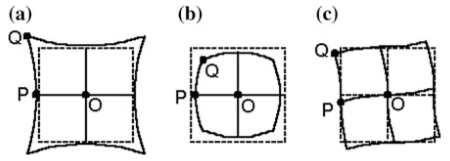
\includegraphics[width=10cm]{pictures/pictures_ch2/Distortions.png}
	\caption{Common types of distortions \cite[p.29]{EGERTON_2016}}
	\label{fig: commonDistortions}
\end{figure}

\subsection{Electron Sources}
\subsection{Electron Lenses, Defects and Correction}

In order to focus a light beam, light optics use convex lenses. Electron optics is based on similar principles of image formation. The equivalent of an convex lens in light optics are either electrostatic or magnetic lenses in electron optics. using either electrostatic or magnetic fields to deflect the electron's trajectories.\\

The simple arrangement of an electrostatic lens could be described as a circular conducting electrode with a circular hole for the optic axis. The circular electrode is further connected to a negative voltage and hence electrons passing the hole with a trajectory not lying on the optic axis are repelled by the non-uniform electric field. The deflection angle hence depends on the displacement from the optic axis. For the purpose of focusing, the formation of a point image can be expected out of the electrons originating from point source as pictured in figure \ref{fig: unipotentialLens}. In particular, the electrostatic lens in figure \ref{fig: unipotentialLens} is known as unipotential lens or einzel lens. Unipotential lenses consist of additional circular electrodes placed before and after the the central electrode to limit the extent of the electric field. This ensures that the electrons leave with the same potential as they enter with. The electrostatic fields further show cylindrical symmetry, hence the focusing force depends only on the radial distance from the optic axis. and is independent of the azimuthal direction around the axis \cite[p.33]{EGERTON_2016}.\\



\begin{figure}[!ht]
	\centering
	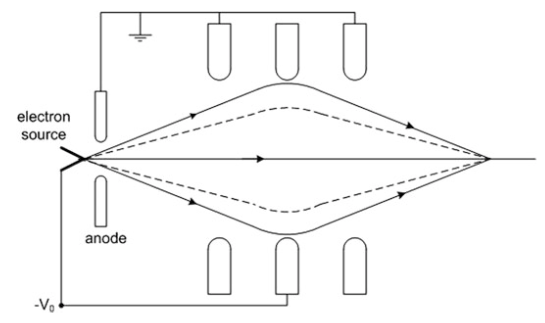
\includegraphics[width=10cm]{pictures/pictures_ch2/UnipotentialLens.png}
	\caption{Unipotential, electrostatic lens \cite[p.33]{EGERTON_2016}}
	\label{fig: unipotentialLens}
\end{figure}

\newpage